% Chapter 1

\chapter{Perspectives Towards Critical Heat Flux Prediction} % Chapter title

\label{ch:to_CHF} % For referencing the chapter elsewhere, use \autoref{ch:introduction} 

\minitoc
%----------------------------------------------------------------------------------------

In this last Chapter of this Part dedicated to the modeling of wall boiling, we briefly discuss historical approaches to represent the Boiling Crisis and propose a perspective use of Heat Flux Partitioning models as a mean to estimate the Critical Heat Flux.


\section{Previous Modeling of the Boiling Crisis}

Historically, since the pioneering observations of Nukiyama \cite{nukiyama_maximum_1966} who identified the maximum boiling heat flux, the question of explaining the triggering of the Boiling Crisis has been thoroughly investigated by many researchers who attempted to propose various physical explanations and modelings aimed to estimate the value of the CHF.


\subsection{Empirical Approaches}

As a direct way of estimating the CHF, empirical approaches have remained the preferred solution for engineering problems to tackle the Boiling Crisis issue. Indeed, according to Groeneveld \cite{groeneveld_2006_2007}, more than 1000 dedicated CHF correlations for water and heated tubes were reported in 2007. As mentioned in the Introduction (Chapter \ref{ch:introduction}), current safety analyses in the nuclear industry actually rely on specific correlations tied to a given core / fuel assembly geometry and usually depend on the pressure $P$, the mass flux $G$, the inlet quality $x_{eq,in}$ and geometry through the thermal /heated diameter $D_{th}$ and distance between the mixing grids $L_{g}$. For instance, Westinghouse company developed the so-called "Tong-67" correlation \cite{tong_prediction_1967} based on data-fitted optimization. 

\npar

Following the huge number of CHF experimental tests that were conducted over the past decades, Groeneveld \etal \cite{groeneveld_2006_2007} proposed to simply gather a very large number of measurements in order to come up with a "Look-Up Table", which directly tabulates the CHF values depending on the operating conditions. Though computationally efficient, this approach is not extendable to any other conditions except those covered by the table data. As a result, their work is limited to external upward flow of water around circular tubes (\eg fuel rods).  


\subsection{Physical Phenomenology Approaches}


In 1948, Kutateladze \cite{kutateladze_transition_1948} proposed a dimensional analysis to tackle the question of the boiling crisis. Stating that near CHF, the concept of single bubbles / nucleation sites behaviors is lost, he considered the boiling crisis to come from the destruction of stability of two-phase flow existing near the wall. Based on the interaction of three "energetic scales" respectively associated to surface tension force, gravity and turbulence, he derived:

\begin{equation}
\phi_{w,CHF} = C_{K} h_{LV} \rho_{V} \parth{\frac{\sigma \parth{\rho_{L} - \rho_{V}}g}{\rho_{V}^{2}}}^{1/4}
\label{eq:chf_kutateladze}
\end{equation} 
where $C_{K}=0.16$ was obtained from experiments.

\npar

This formulation of the CHF found a true success due to its analytic nature and its good performance for moderate to high pressure measurements. The coherent behavior of Kutateladze law has been once more recently confirmed by Kossolapov \cite{kossolapov_experimental_2021} whose CHF measurements dependency with pressure were fairly reproduced.

\npar

Kutateladze approach was further developed by Zuber \cite{zuber_hydrodynamic_1959} who proposed a physical interpretation of the  Boiling Crisis as an hydrodynamic instability. Considering vapor columns coming out of the heated surface (Figure \ref{fig:chf_zuber}), he supposed that the Boiling Crisis was triggered under a combination of Rayleigh-Taylor and Kelvin-Helmoltz instabilities. Assuming the vapor columns were regularly spaced by a distance equal to the Rayleigh-Taylor instability wavelength, the Boiling Crisis is supposed to be triggered by the merging of those vapor columns due to the emergence of Kelvin-Helmholtz instabilities. He then could analytically derive:

\begin{equation}
\phi_{w,CHF} = \frac{\pi}{24} h_{LV} \rho_{V} \parth{\frac{\sigma \parth{\rho_{L} - \rho_{V}}g}{\rho_{V}^{2}}}^{1/4} \parth{ \dfrac{\rho_{L} }{\rho_{L} + \rho_{V}} }^{1/2}
\label{eq:chf_zuber}
\end{equation} 
which degenerates to Kutateladze formulation when $\rho_{L} \gg \rho_{V}$ with the constant value $C_{K} = \pi / 24 \approx 0.131$.

\begin{figure}[!h]
\centering
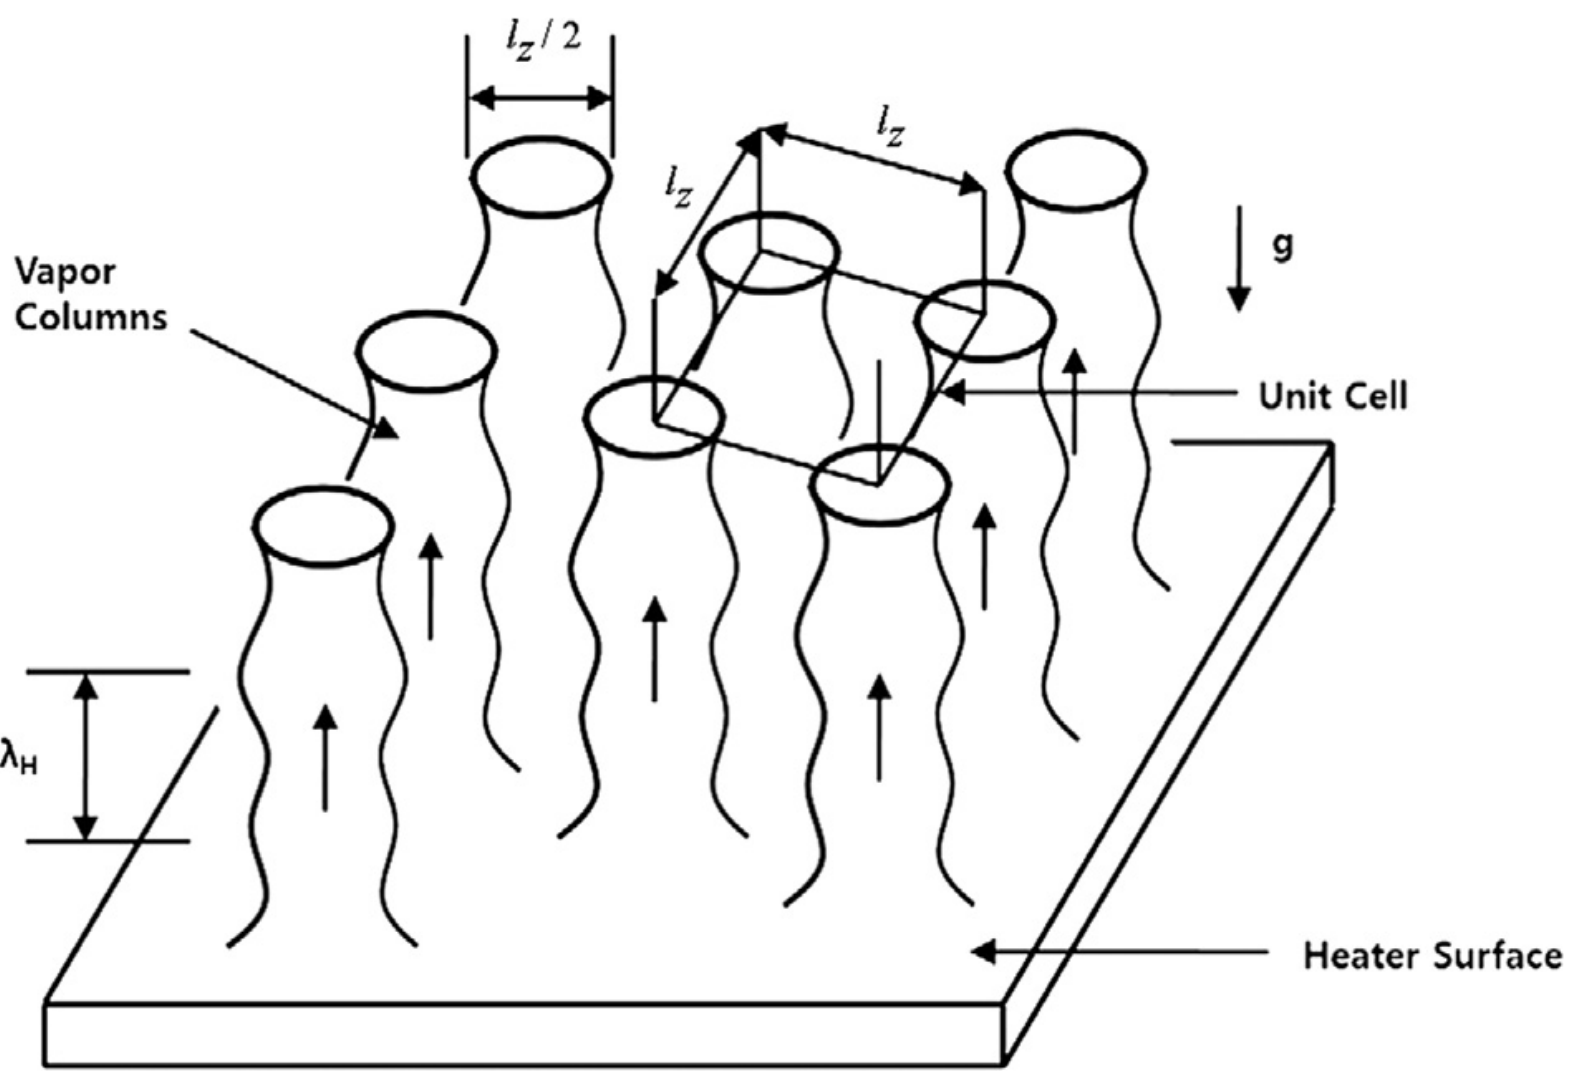
\includegraphics[width=0.6\linewidth]{img/chf/chf_zuber.png}
\caption{Sketch of the boiling crisis description by Zuber \cite{zuber_hydrodynamic_1959}. $l_{z}$ and $\lambda_{H}$ are respectively the Rayleigh-Taylor and Kelvin-Helmholtz instability wavelengths.}
\label{fig:chf_zuber}
\end{figure}


\begin{note*}{}
The formulations of Kutateladze and Zuber were both derived for horizontal pool boiling.
\end{note*}

\npar


Other approaches are based on different physical mechanism. For instance, Lee \& Mudawar \cite{lee_mechanistic_1988} propose to describe the boiling crisis phenomenon as the evaporation of a very thin liquid layer trapped between the wall and an elongated slug of vapor (Figure \ref{fig:chf_lee}), following experimental observations %\cite{Mesler (1976), Molen  Galjee (1978), Bhat et al. (1983), Serizawa
%(1983), Hino  Ueda (1985) and Mudawwar et al. (1987)}.

\begin{figure}[!h]
\centering
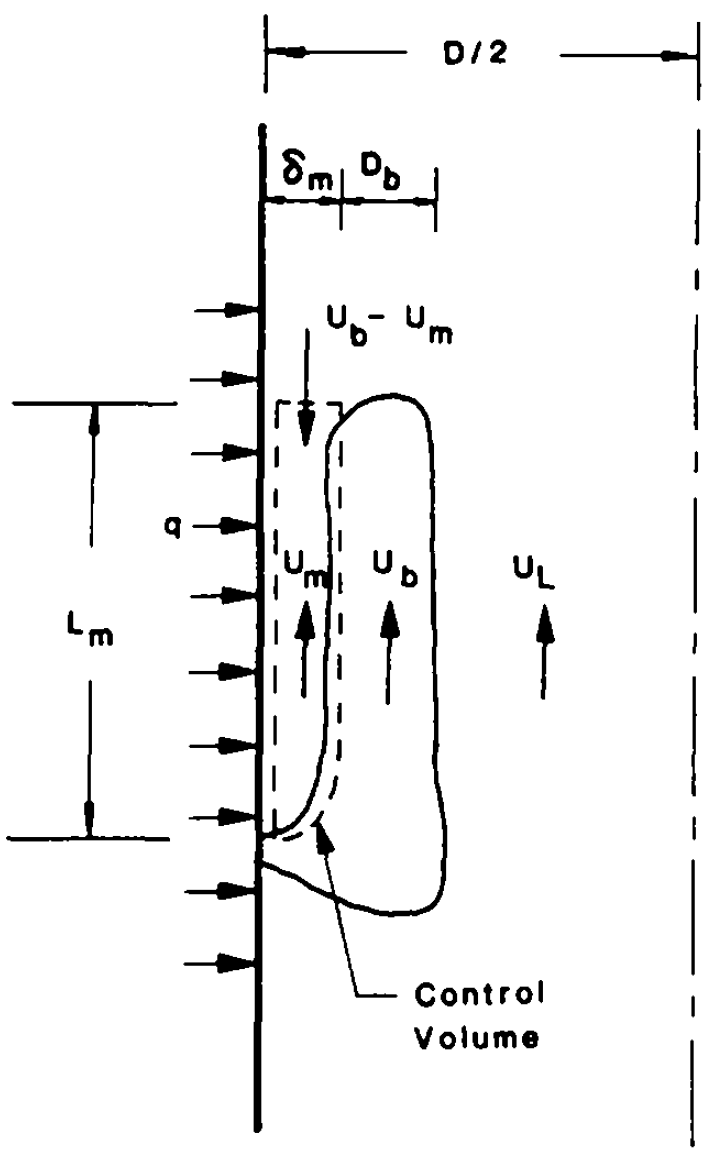
\includegraphics[width=0.4\linewidth]{img/chf/chf_lee.png}
\caption{Sketch of the boiling crisis description by Lee \& Mudawar. Here, the boiling crisis is supposed to be triggered when the evaporation rate of the sublayer exceeds the entering liquid flux (\ie when velocity $U_{b}-U_{m}$ approaches 0).}
\label{fig:chf_lee}
\end{figure}

\npar

The idea that the boiling crisis is associated to rapid dynamics of bubble base evaporation was also explored by Nikolayev \& Beysens \cite{nikolayev_boiling_1999} who considered the force exerted by the vapor recoil at the bubble base during boiling. They found that this force could trigger a change in bubble shape through a change of the apparent contact angle, leading to the irreversible growth of the dry area. This was further confirmed at low-gravity conditions for liquid helium near the critical temperature \cite{nikolayev_experimental_2006, nikolayev_boiling_2015}.


\npar

On the other hand, Weisman \& Pei \cite{weisman_prediction_1983} proposed that the boiling crisis was due to lack of turbulent transport of the bubbles from the wall towards the bulk, resulting in a bubble layer close to the wall (Figure \ref{fig:chf_weisman}) that will trigger coalescence near the heater and isolating it from the liquid phase. 



\begin{figure}[!h]
\centering
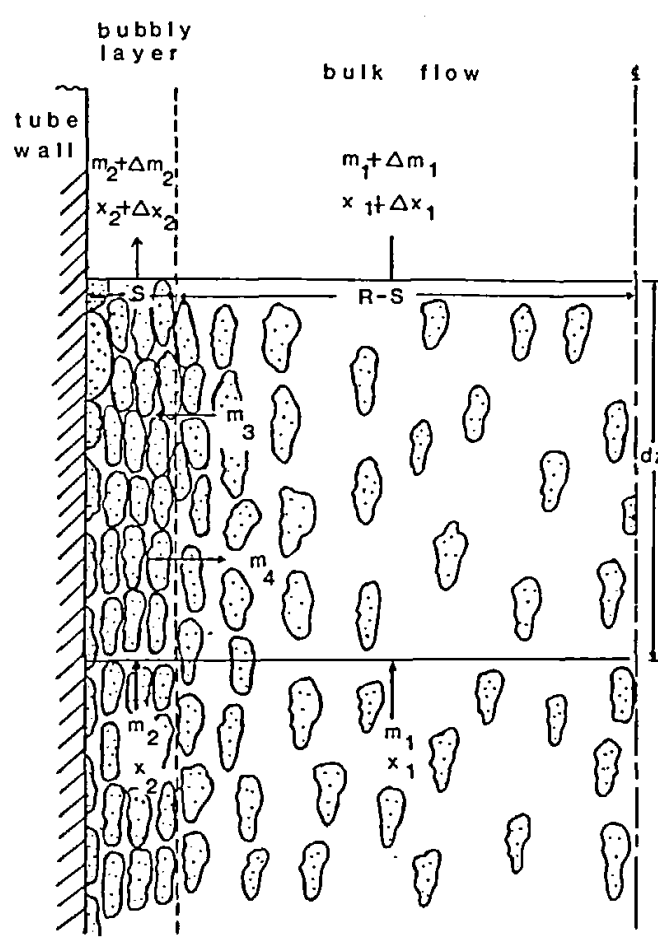
\includegraphics[width=0.4\linewidth]{img/chf/chf_weisman.png}
\caption{Sketch of the boiling crisis description by Weisman \& Pei}
\label{fig:chf_weisman}
\end{figure}

\npar

Assuming bubbles were of ellipsoidal shapes at CHF, they considered that boiling crisis occurred when the maximum packing density was reached, \ie having a wall void fraction:

\begin{equation}
\alpha_{CHF} = 0.82
\end{equation} 

Although this criterion is very suitable for CMFD applications \cite{mimouni_computational_2016, liu_critical_2021}, the critical void fraction close to the wall can vary in large ranges (down to 30\% at high subcooling) according to experimental observations \cite{bruder_empirical_2018}.


\section{Recent Approaches and Advances for CHF Prediction}



The question of the boiling crisis occurrence and CHF value is still a topic of active research nowadays. Recently, new experimental observations have allowed the access to wall-related boiling measurements \cite{kossolapov_experimental_2021, richenderfer_experimental_2018, bloch_study_2016} and permitted to better understand the phenomenology behind the trigger of the boiling crisis.

\npar

\subsection{Dry Patch Formation}

As detailed by Kossolapov \cite{kossolapov_experimental_2021}, a significant number of different experiments studying the wall boiling at CHF have demonstrated that the occurrence of the boiling crisis was similar at various pressures and associated to the formation of an irreversibly growing dry patch \cite{kossolapov_experimental_2021, richenderfer_experimental_2018}. Such observations are leveraging mechanistic behavior of bubbles right before the CHF. First attempts of modeling this phenomenon were proposed by Ha \& No \cite{ha_dry-spot_1998}, prior to the aforementioned experimental observations. Based on a random distribution of the bubbles on the heater surface (similar to the Poisson distributions discussed in Section \ref{sec:site_interactions}), they proposed that a dry patch is created when a bubble crowding hindering rewetting is reached, which was translated as:

\begin{equation}
\phi_{w} = \phi_{1b}N_{sit,a} \parth{1 - \mathcal{P}\parth{N \geq N_{c}}}
\end{equation}
where $\mathcal{P}\parth{N \geq N_{c}}$ is the probability to find more than $N_{c}$ bubbles in the area of influence of a single bubble and $\phi_{w,1b}$ is the heat flux removed by a single bubble.

\npar

They noted that this ponderation of the total heat flux allowed to reach reasonable predictions of the maximum heat flux when $N_{c}=5$ (Figure \ref{fig:chf_ha}).



\begin{figure}[!h]
\centering
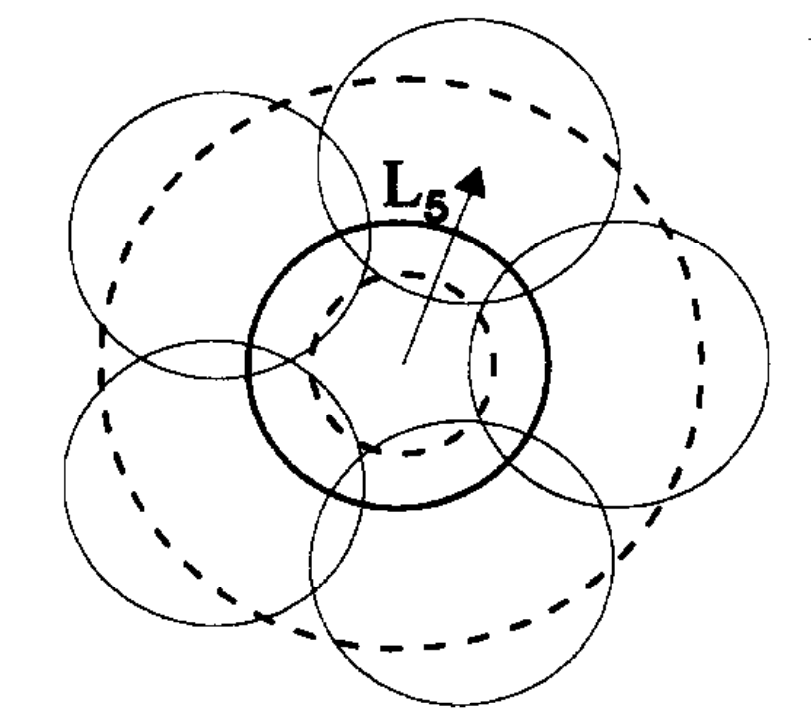
\includegraphics[width=0.35\linewidth]{img/chf/chf_ha.png}
\caption{Sketch of the dry patch formation mechanism by and adapted from Ha \& No \cite{ha_dry-spot_1998}.}
\label{fig:chf_weisman}
\end{figure}


This model was recently re-used by Dong \& Gong for low pressure cases \cite{dong_numerical_2022}.



\subsection{Model of Baglietto, Demarly \& Kommajosyula \cite{baglietto_boiling_2019} : Stability of the Heat Flux Partitioning}

In the framework of Heat Flux Partitioning modeling of Kommajosyula \cite{kommajosyula_development_2020} and Demarly \cite{demarly_new_2020}, Baglietto \etal \cite{baglietto_boiling_2019} proposed a modeling of the wall area in direct contact with vapor (corresponding to $A_{c,V}$ in Section \ref{sec:hfp_new}). Over the direct area beneath single bubbles, they account for bubble interaction and models the total wall dry are $S_{dry}$ as:

\begin{equation}
S_{dry} = ft_{g,d} N_{sit,a} \pi \parth{\zeta \underbrace{ e^{f t_{g,d}N_{sit,a} \pi R_{d}^{2} } }_{\text{Bubble interaction}}  \sin{\theta} R_{d} }
\end{equation} 
where $\zeta=0.15$ based on data-fitting of Richenderfer \cite{richenderfer_experimental_2018} experiments.

The total heat flux is finally written as:

\begin{equation}
\phi_{w}=\parth{1-S_{dry}}\parth{\phi_{c,L} + \phi_{e} + \phi_{q}} + S_{dry} \phi_{dry}
\end{equation}
where $\phi_{dry}$ is the heat flux through the dry area, which is nearly negligible versus the other heat fluxes.

\npar

This modeling allows to impose a decrease of the total heat flux by gradually enhancing the growth of the dry area, thus inducing a decrease of $\phi_{w}$ when covering a whole boiling curve (Figure \ref{fig:chf_baglietto}).

\begin{figure}[!h]
\centering
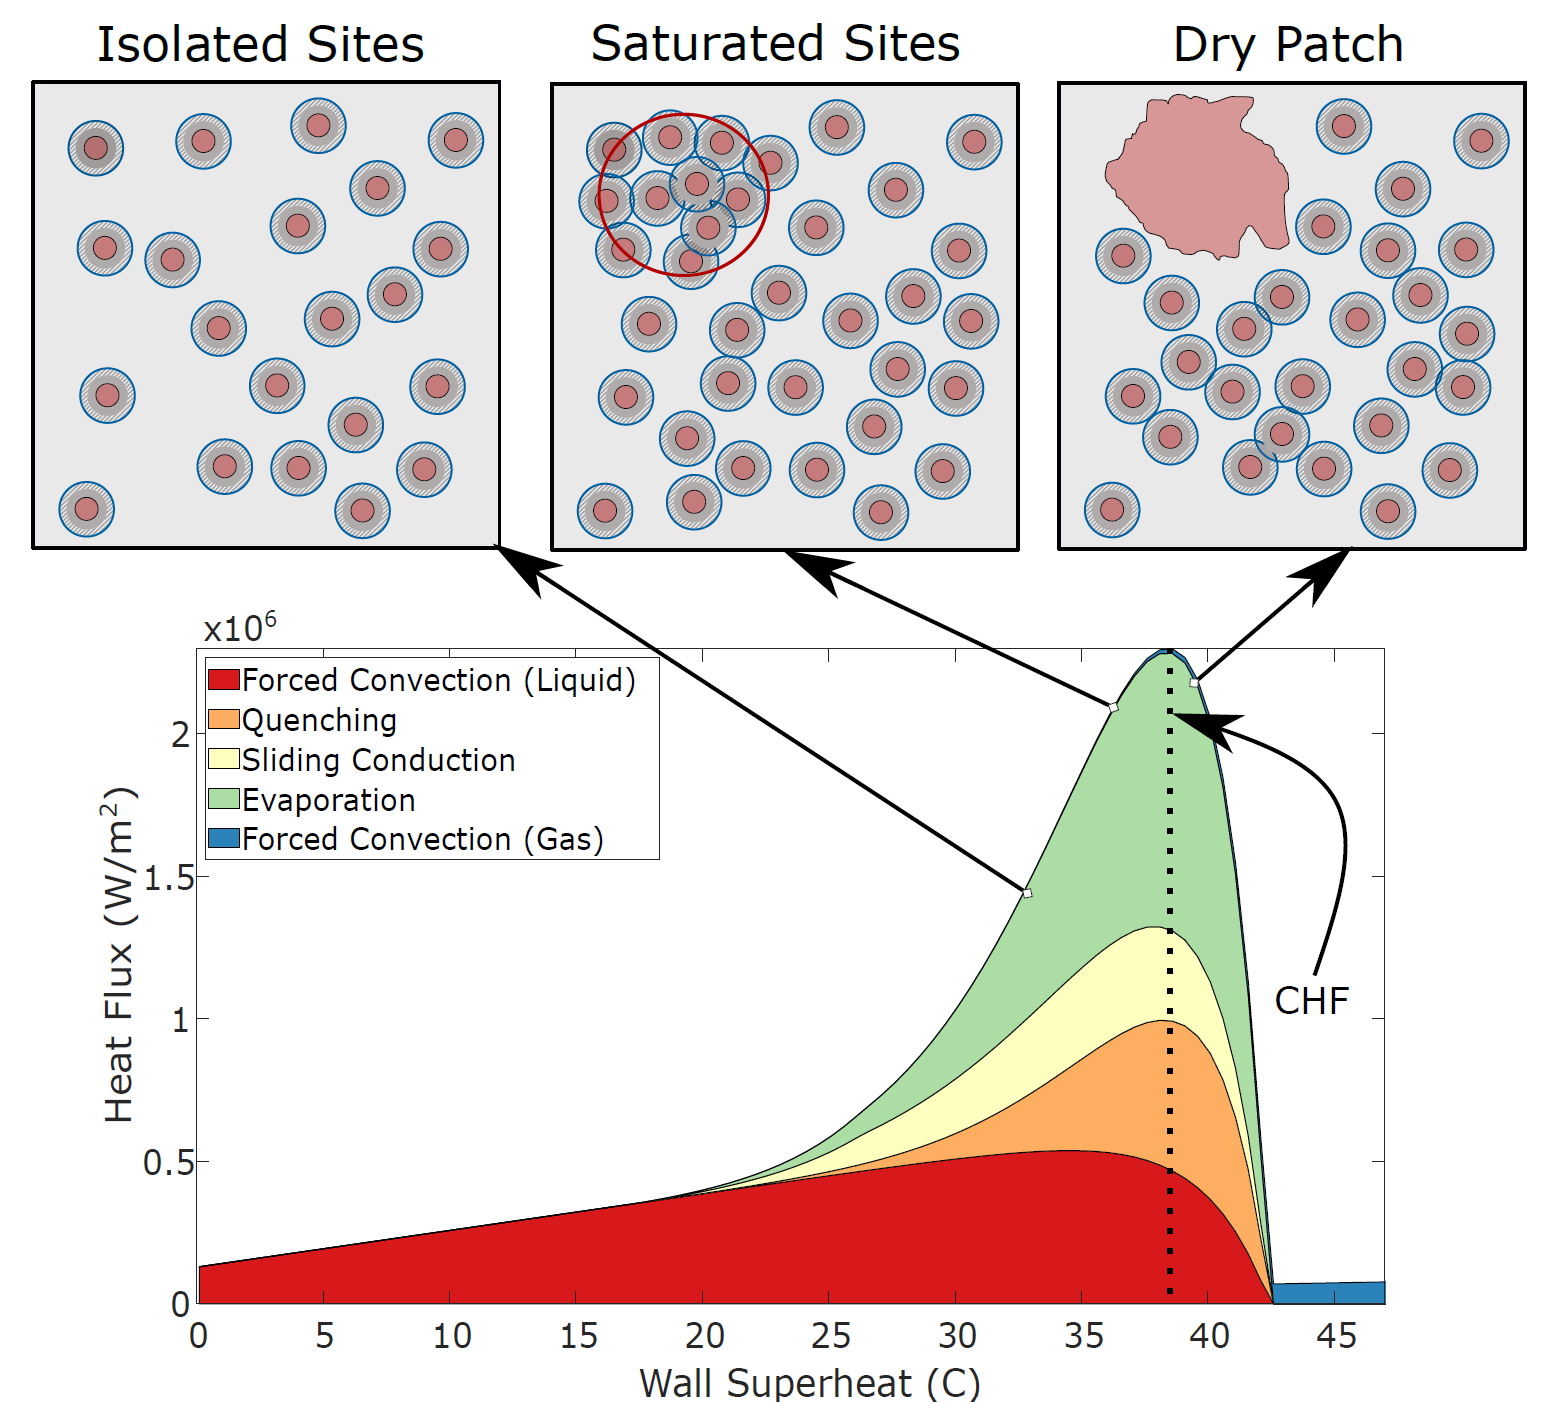
\includegraphics[width=0.6\linewidth]{img/chf/chf_baglietto.png}
\caption{Illustration of CHF prediction by Baglietto \etal \cite{baglietto_boiling_2019}.}
\label{fig:chf_baglietto}
\end{figure}

This model was applied for both low and high pressure cases by Demarly \cite{demarly_new_2020} and predicted most CHF values within a $\pm 30\%$ error.

\begin{remark*}{}
Since this model detects the CHF as the maximum value reached for $\phi_{w}$ on the boiling curve, its application requires to compute the heat flux partitioning for a large enough range of wall superheat and then extract the maximum $\phi_{w}$ resulting from the computation. 

\npar

For CFD applications, this requires to apply this procedure in each cell to obtain the local value of the CHF, which would result in the possibility of estimating the local DNB ratio (Section \ref{sec:intro_chf_indus}) in a way similar to current industrial approaches.
\end{remark*}



\subsection{Model of Zhang, Seong \& Bucci \cite{zhang_percolative_2019}:  Bubble Interaction and Scale-Free Footprint distribution}



Based on experimental observations, Zhang \etal \cite{zhang_percolative_2019} have observed that the boiling crisis behaved as a scale-free phenomenon by tracking the distribution of bubble footprint area. In particular, they noted that bubble clustering on the surface could be used as an indicator for boiling crisis occurrence: when following the size of the two largest clusters of bubbles, CHF was attained when the second largest cluster reached its maximum size.

\npar

Moreover, they managed to reproduced the bubble footprint power-law distribution with a simple Monte-Carlo stochastic simulation (Figure \ref{fig:chf_zhang_cluster}), using measured physical inputs being the average bubble radius $\left<R\right>$, active nucleation site density $N_{sit,a}$ and probability of finding a bubble on the surface $t_{g}f$.

\begin{remark*}{}
This power-law for the probability density function of bubble dry area distribution, becoming critical near CHF, has been further confirmed by Kossolapov \cite{kossolapov_experimental_2021} who found same distributions at various pressures up to $75\ $bar.
\end{remark*}

\begin{figure}[!h]
\centering
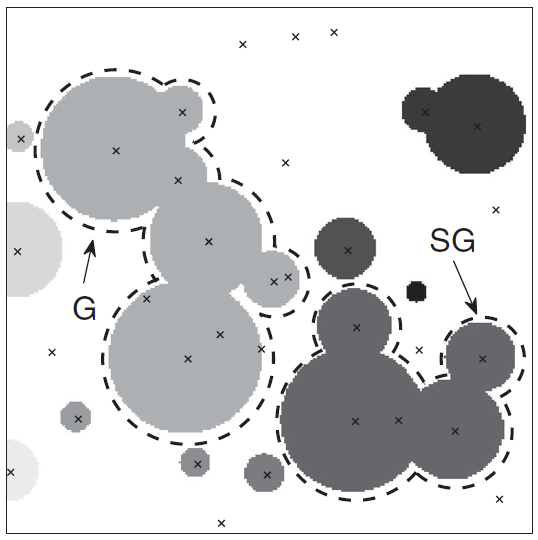
\includegraphics[width=0.35\linewidth]{img/chf/chf_zhang_cluster.png}
\caption{Example of Monte-Carlo simulation of the bubble clustering process, by and adapted from \cite{zhang_prl}. $G$ and $SG$ respectively denote the largest and second largest bubble clusters.}
\label{fig:chf_zhang_cluster}
\end{figure}

\npar

Further investigating these findings, Zhang \cite{zhang_new_2022} concluded that the computed CHF was mostly controlled by the values of the three physical input parameters:  $\left<R\right>$, $N_{sit,a}$ and $t_{g,d}f$. Her idea was then to suppose that the boiling crisis could be detected based only on this so-called "triplet". This has been further confirmed through the work of Ravichandran \etal \cite{ravichandran_online_2019, ravichandran_infrared_2022} who used neural-networks for real-time processing of boiling experiments. While trying to tentatively anticipate the CHF value in given operation conditions, they showed that most of the information regarding the CHF prediction with the neural-network was contained in the three values $\left<R\right>$, $N_{sit,a}$ and $t_{g,d}f$ by reaching nearly 90\% of prediction accuracy.

\npar

Experiments presented in Zhang PhD \cite{zhang_new_2022} finally demonstrated this capacity of CHF anticipation. By covering 11 different heater material / fluid combinations in both pool and flow boiling, boiling crisis occurred every time when:

\begin{equation}
N_{sit,a} \pi \left<R\right>^{2} t_{g}f \sim 1
\label{eq:chf_zang}
\end{equation}

This dimensionless relationship physically means that non-interacting bubbles cover in average the entire boiling surface, which seems reasonable when approaching the boiling crisis.


\section{Simple test of the Zhang Criterion}

The criterion proposed by Zhang in the last sub-section presents a particular interest in the frame of HFP models. Indeed, it relies on physical parameters that are all computed in the Heat Flux Partitioning process, namely the average bubble radius $\left<R\right>$, the bubble-generating sites density $N_{sit,a}$, the bubble growth time  $t_{g}$ and nucleation frequency $f$. 

\npar

Regarding CFD application, this results in a very simple value to compute in every wall boiling cells in order to estimate the local proximity to the boiling crisis. As a prospective test, we computed this value using the original NEPTUNE\_CFD HFP formulation (Section \ref{sec:ncfd_HFP}) on a DEBORA case (Figure \ref{fig:debora_chf_criterion}).

FIGURE CHF CRITERION DEBORA


\npar

First, we must acknowledge that the values of the CHF criterion $N_{sit,a} \pi \left<R\right>^{2} t_{g}f$ are not calibrated to reach of value around 1 at the CHF since the initial HFP model of NEPTUNE\_CFD presents obsolete closure laws (Chapter \ref{chap:HFP_Assembling}). However, we can qualitatively study the evolution of the criterion value by logically considering that the higher the CHF triplet, the closer we locally are to the boiling crisis.

\npar

From that, we can observe that for the simple DEBORA case, the value of the criterion progressively rises as we move upwards the heating length. Qualitatively, it indicates that the longer we heat the closer we are to the boiling crisis, which is physically expected. 

\npar

At first glance, this criterion thus seems to present a reasonable qualitative behavior and may be more relevant than local wall temperature (which is nearly constant in the whole boiling region) or void fraction (strongly depending on the mesh size if taken at the wall cell).

\begin{remark*}{}
Testing this criterion with new model using the wall liquid properties extracted from the CFD simulations resulted in an outlet value of $N_{sit,a} \pi \left<R\right>^{2} t_{g}f \approx 0.83$ which falls better in the range of [0, 1] found by Zhang.
\end{remark*}


\section{Conclusions}

In this prospective Chapter, we presented former approached for CHF estimation and discussed the possibility of achieving boiling crisis prediction using the Heat Flux Partitioning Modeling framework. Finally, we can note that:

\begin{itemize}
\item Recent experimental observation from various authors are starting to reach a general agreement regarding the physics of Departure from Nucleate Boiling, where wall boiling measurements showed that boiling crisis coincides with the formation of an irreversible dry patch

\item The modeling of the dry wall area has thus been studied by Baglietto \etal \cite{baglietto_boiling_2019} who managed to display a maximum wall heat flux by accounting for bubble interactions.

\item Further experimental studies of Zhang \etal \cite{zhang_percolative_2019}, Zhang \cite{zhang_new_2022} and Kossolapov \cite{kossolapov_experimental_2021} showed that the boiling crisis seems intrinsically linked to bubble footprint distribution becoming critical at CHF.  

\item Zhang \cite{zhang_new_2022} and Ravichandran \etal \cite{ravichandran_infrared_2022} showed that those latter observations were strongly depending on the physical triplet ($\left<R\right>$, $N_{sit,a}$, $t_{g}f$) which proved to be sufficient to predict boiling crisis occurrence when $N_{sit,a} \pi \left<R\right>^{2} t_{g}f \sim 1$.

\item Test of this last criterion was very suitable for CFD application using Heat Flux Partitioning approach and showed a coherent qualitative behavior on a simple tube case from the DEBORA database.
\end{itemize}
